\documentclass[a4paper, openany]{memoir}

\usepackage[utf8]{inputenc}
\usepackage[T1]{fontenc} 
\usepackage[english]{babel}
\usepackage{amsmath}
\usepackage{amssymb}

\usepackage{booktabs}
\usepackage{fancyhdr}
\usepackage{float}
\usepackage{indentfirst}
\usepackage{graphicx}
\usepackage[linewidth=1pt]{mdframed}
\usepackage{multicol}
\usepackage{fancyvrb}

\pagestyle{fancy}
\fancyhf{}
\fancyhead[LE]{\leftmark}
\fancyhead[RO]{\rightmark}
\fancyhead[RE, LO]{PSD}
\fancyfoot[LE, RO]{\thepage}
\fancyfoot[RE, LO]{Pete Gautam}

\renewcommand{\headrulewidth}{1.5pt}

\chapterstyle{thatcher}
\setcounter{chapter}{10}

\begin{document}

\chapter{Behaviour Driven Development}
In Behaviour driven development (BDD), we implement the software by prescribing its behaviour and testing whether it matches the expected behaviour. There are 3 terms used to describe tests:
\begin{itemize}
    \item A test case describes a set of actions to be performed on the software, along with the expected outcome.
    \item A test is the execution of a test case, which results in a test outcome.
    \item Testing is the practice of creating, maintaining, executing and evaluating test cases.
\end{itemize}

There are many reasons for using a test-driven approach in software development. The oldest, and the classic reason to do this is to detect defects. We use tests to check whether the implementation matches the high-level description of how the system is supposed to behave. This practice is still present, particularly where there is a need to show the independence of testing for audit purposes. However, in small teams, there are other reasons that are more important. These are:
\begin{itemize}
    \item to support the design and the implementation of a module using practices such as test and behaviour-driven development.
    
    \item to prevent the introduction of defects, particularly if these tests are used as part of an automated test suite in a CI pipeline.
    
    \item to document the behaviour of a system, where it can be used to demonstrate the interactions that can be performed on a system API.
    
    \item to demonstrate that a system meets its specification.
\end{itemize}

\section{Scales of testing}
There are 3 scales of testing- unit tests, integration tests and acceptance tests. A mature application will likely have a very large suite of unit tests. A unit test focuses on checking the behaviour of a single module, such as a class. Since there could be a lot of unit tests, we expect their execution to be quite fast. So, unit test cases should use test doubles (such as fakes and mocks) and avoid performing slow activities (such as input and output).

Acceptance (or system) tests are performed on a fully integrated system. These are relatively costly, e.g. they might interact with external resources. An application will have a smaller number of acceptance tests cases. These are used to show that the system meets its specification and document use cases. Acceptance tests can be manually executed by an operator on an interface at a set of phrases during the project's lifecycle. It is often more expensive to maintain an automated acceptance test for it than for it to be performed manually. We treat non-functional properties (e.g. speed of execution) as acceptance test cases. They cannot be properly evaluated if some components are replaced with doubles.

Integration test lies between unit and acceptance testing. It is used when integrating subsets of the system's components. However, we still use test doubles at this level since we are testing an incomplete system.

\section{BDD and acceptance testing}
BDD involves creation and maintenance of a requirements specification in a structured, natural language (called Gherin). From the requirements, we create test cases automatically. Using these test cases, we can test whether the actual implementation matches the expected result.

Requirements can be expressed as user stories and the scenarios derived from the stories. An example of a user story/scenario is given below:
\begin{verbatim}
Feature: manage account balance
  As a bank account holder
  I want to make transactions on my bank account
  So that I can manage my finances

  Scenario: deposit an amount into the account.
    Given a bank account for "Alice"
    When I deposit 100 GBP into the bank account for "Alice"
    Then the bank account for "Alice" balance should be 100 GBP
\end{verbatim}
\noindent This is an example of a specification by example. User stories provide high level outline for a feature. Scenarios provide a use case of that feature. 

Language concepts should refer to the problem domain in a feature instead of the technical domain. That is, we should not use programming concepts in user stories and scenarios (e.g. exceptions).

BDD provides a technical infrastructure for explicitly linking these artifacts to an implementation. In principle, maintaining explicit links between requirements specification, test cases and implementation allows the features to be demonstrated in a corresponding implementation. We demonstrate the implementation to the users in Gherkin.

BDD is generally used for writing acceptance test cases in order to support the design of the system with users. It is used to demonstrate that the implementation meets the specification and to document the behaviour of the system. It could be used for unit and integration test cases, but this has a huge overhead and isn't typically worth it.

Nonetheless, BDD test cases can be executed automatically. So, it can be used to detect regression (i.e. introduction of defects). However, it is technically used to describe system tests. This means that it is harder to determine the cause of a failed test using BDD. In particular, it is difficult to isolate the defect using a BDD test case in comparison to a suite of very finely defined unit test cases.

\section{BDD lifecycle}
The following image gives the lifecycle of BDD.
\begin{figure}[H]
    \centering
    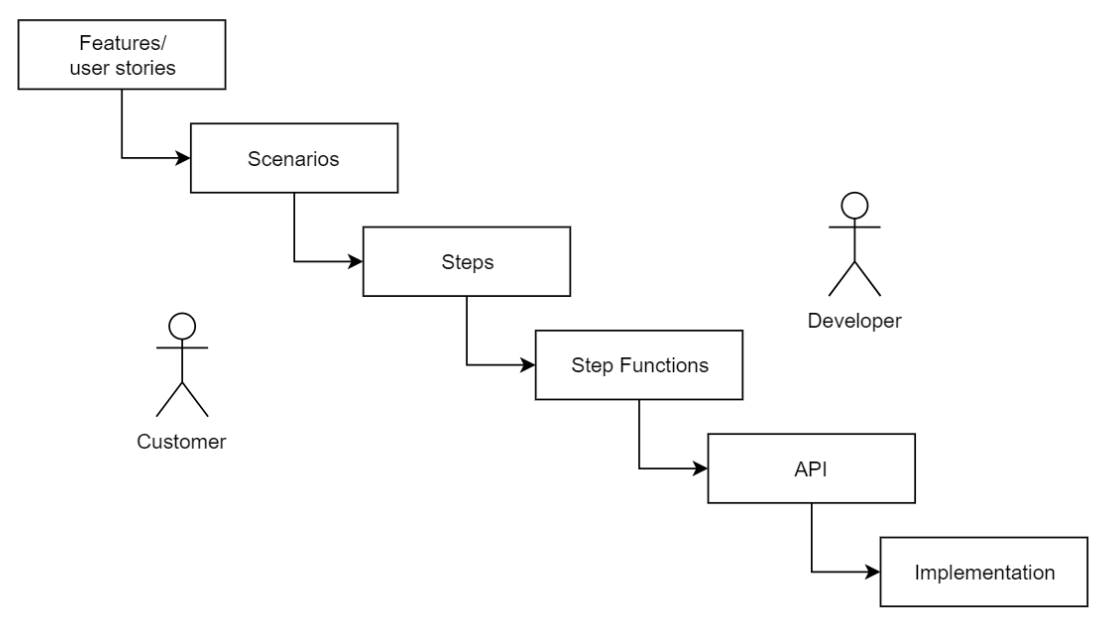
\includegraphics[scale=0.5]{src/11 BDD Lifecycle.PNG}
    \caption{The BDD Lifecycle.}
\end{figure}
\noindent There are many stages to BDD, which we highlight below:
\begin{itemize}
    \item First, the features of the system are outlined as user stories. This can be done in a user story workshop, which is a way for customer, developers and users to collaborate and produce user stories.
    
    \item Then, we develop scenarios that show different use cases for a feature.
    
    \item Next, we add individual steps for each scenario, which get translated into the target application language as step functions. These drive the design of the API and then its implementation.
\end{itemize}

As we can see, the diagram looks like the waterfall method. In fact, the only difference is that testing takes place before implementation. For this reason, this method does not work in practice. It is much more feasible to develop features concurrently with implementation. This avoids too much top-down design. This is particular useful when the feasibility of a proposed design and constraints imposed by dependencies are unknown. 

Nonetheless, the diagram above is still useful. It still shows the hierarchical relationship between high-level user stories to the intermediate artifacts (i.e. steps and step functions), followed by the underlying implementation.

\subsection{Steps}
In Gherkin, scenarios are divided into 3 types of steps:
\begin{itemize}
    \item a \texttt{given} step, which describes how to set up the text case fixture.
    \item a \texttt{when} step, which lists actions to be taken during the test case.
    \item a \texttt{then} step, which is composed of assertions that are made about the state of the system at the end of the case.
\end{itemize}

Consider the example below of a Gherkin scenario.
\begin{verbatim}
Given a bank account,
When I deposit 100 GBP into the bank account,
Then the bank account balance should be 100 GBP.
\end{verbatim}
It has a given, when and a then step. It can be realised as a test in Python as shown below.
\begin{figure}[H]
    \centering
    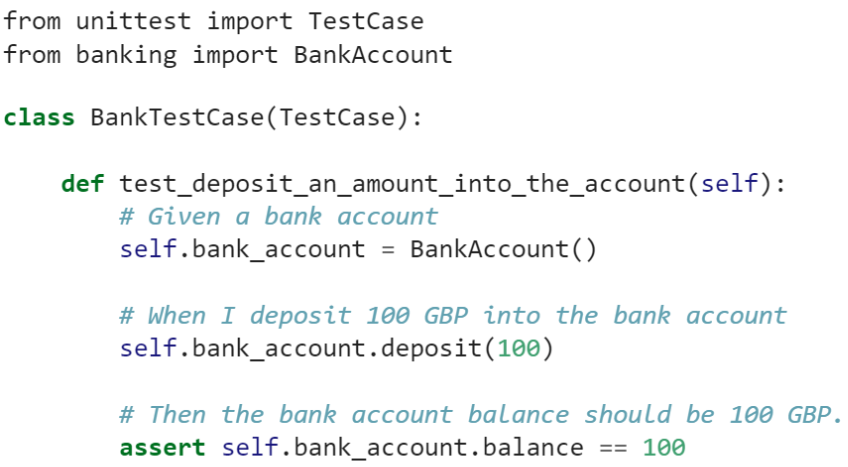
\includegraphics[scale=0.6]{src/11 BDD Python naive test.PNG}
\end{figure}
\noindent Using this, we can implement the class, ensuring that the test cases will pass.
\begin{figure}[H]
    \centering
    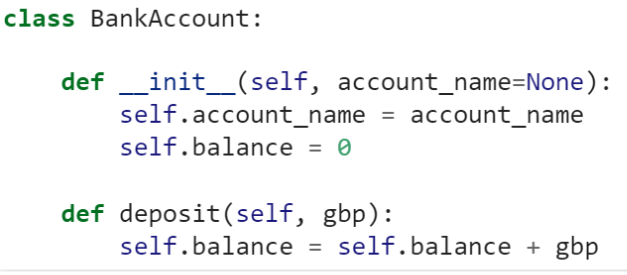
\includegraphics[scale=0.6]{src/11 BDD Python implementation.PNG}
\end{figure}

It can be tedious to map scenarios to test cases. It is likely that there will be a lot of repetition. In particular, the same step may appear in many scenarios, or even get repeated within the same scenario. We can mitigate this by refactoring each step into an individual method, as shown below.
\begin{figure}[H]
    \centering
    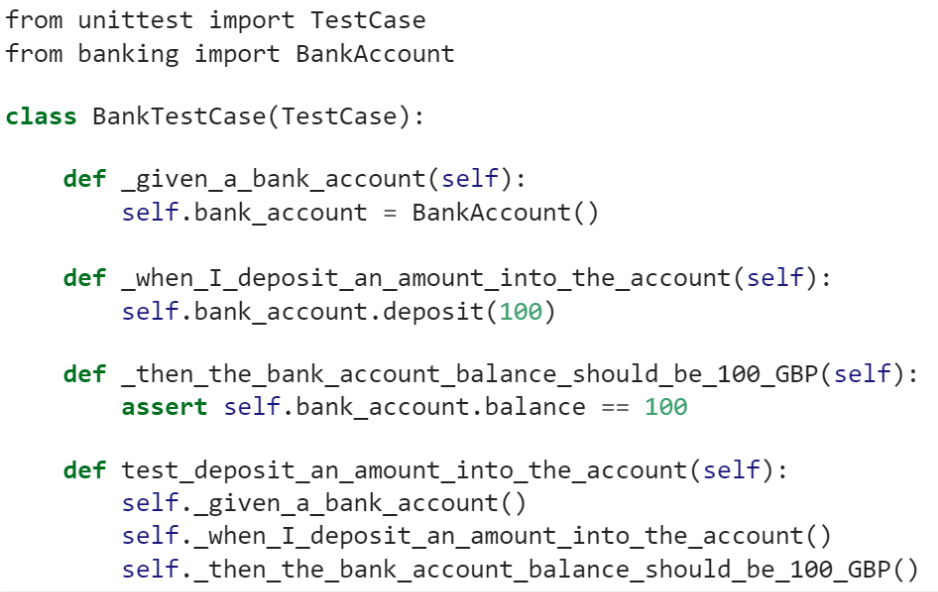
\includegraphics[scale=0.6]{src/11 BDD Python refactored test.PNG}
\end{figure}
\noindent We can now combine the different steps as required to create test cases.

However, we still have to maintain the order in 2 places- in the original Gherkin scenario and the test case file. Instead, we can make use of BDD frameworks to eliminate the redundancy by allowing Gherkin steps to be linked directly to functions and methods. Below are some BDD frameworks:
\begin{itemize}
    \item JBehave for Java,
    \item Behave for Python,
    \item Cucumber for Ruby, Python, Java, etc.,
    \item Behat for PHP,
    \item Specflow, etc.
\end{itemize}

When using a BDD framework, we create a function for each step definition in the application within the programming language. This way, instead of maintaining test cases corresponding to each scenario, we ensure that there is one step definition for each unique step in the feature file. The BDD framework executes scenarios by selecting the correct step functions to execute in sequence. This is summarised in the diagram below.
\begin{figure}[H]
    \centering
    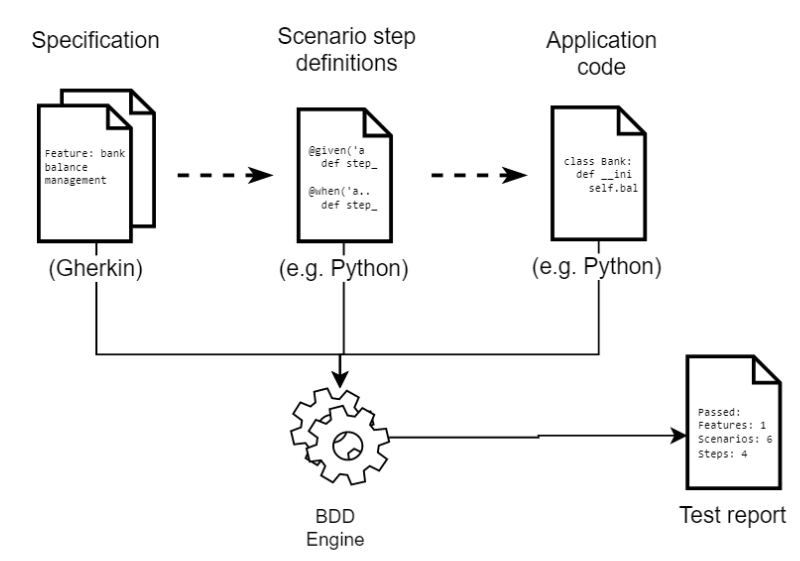
\includegraphics[scale=0.6]{src/11 BDD Framework cycle.PNG}
\end{figure}
\noindent The diagram gives the BDD framework cycle. We take the Gherkin specification, the scenario step definitions in some programming language and the actual code. Then, the BDD engine uses these to produce a test report that summarises how many tests passed.

The step definition file for the Python code above (using Behave) is given below.
\begin{figure}[H]
    \centering
    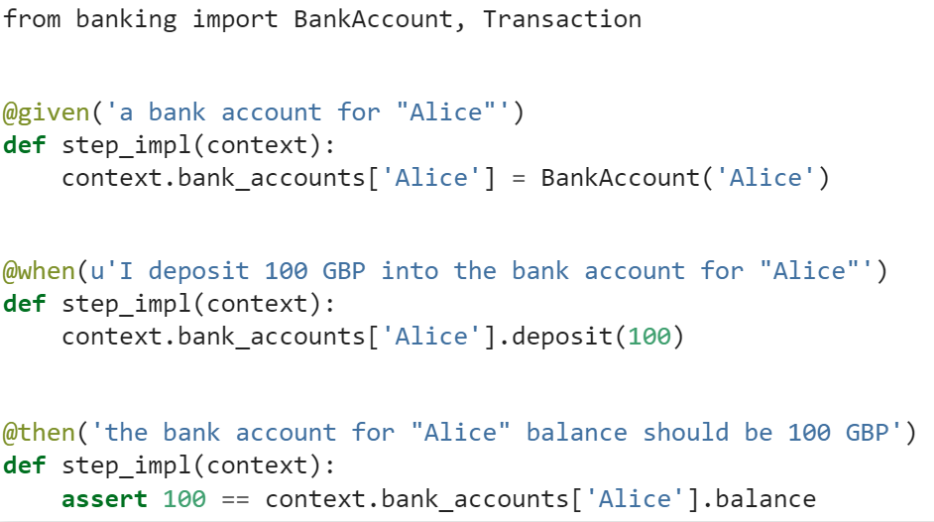
\includegraphics[scale=0.5]{src/11 BDD Python test Behave.PNG}
\end{figure}
\noindent We make use of annotations to identify step definitions along with their descriptions. Then, it produces the test report given below.
\begin{figure}[H]
    \centering
    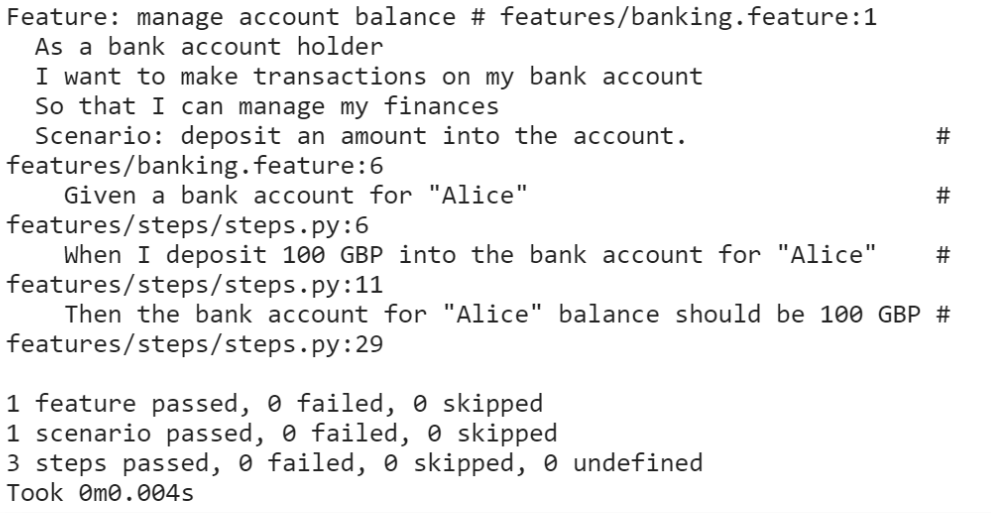
\includegraphics[scale=0.5]{src/11 BDD Python test result Behave.PNG}
\end{figure}

In the particular case of the Python BDD Behave, we start by parsing the Gherkin scenario. It looks up the correct step definition function to execute. It then executes it. Using the shared context, we allow data to be stored between the step functions.

We are using the Facade design pattern here. The module provides methods, each of which implements a more complex functionality in the underlying application. It exposes a high-level method name to the Behave engine. We can do the same in Java, using JBehave.

\subsection{And Steps}
There is a fourth type of step, called the and step. It acts as a synonym for the step type it preceeded. For example, consider the following scenario.
\begin{verbatim}
Scenario: Withdraw an amount from the account.
  Given a bank account for "Alice"
  When I deposit 100 GBP into the bank account for "Alice"
  And I withdraw 50 GBP from the bank account for "Alice"
  Then the bank account for "Alice" balance should be 50 GBP
\end{verbatim}
Here, the and step acts as a when step. By using this style, we make the scenarios user-readable. Also, by following BDD, we will have to explicitly make and document our choices (e.g. how to deal with an overdraft) within the example test cases.

\subsection{Backgrounds}
To not have a lot of duplication within the specifications, we can use backgrounds. This groups steps together that occur in every scenario in a feature. It is executed before the first step in each scenario. An example is given below.
\begin{verbatim}
  Background:
    Given a bank account for "Alice" containing 200 GBP
    And a bank account for "Bob" containing 200 GBP

  Scenario: transaction between two accounts:
    Given a Transaction to transfer 50 GBP from the bank account 
    for "Bob" to "Alice"
    When I execute the transaction
    Then the bank account for "Alice" balance should be 250 GBP
\end{verbatim}

\subsection{Parametrised step functions}
In some cases, we have scenarios that have very similar steps and only different in a few variables. They can be implemented essentially in the same way. For example, consider the following scenarios.
\begin{verbatim}
Scenario: New bank accounts are empty.
  Given a bank account for "Alice"
  Then the bank account for "Alice" balance should be 0 GBP.
\end{verbatim}
\begin{verbatim}
Scenario: Authorised overdraft
  Given a bank account with an overdraft facility of 500 GBP
  When I withdraw 250 GBP from the bank account
  Then the bank account balance should be 250 GBP.
\end{verbatim}

BDD frameworks give us a way to have one step function for each step within these scenarios, where we parametrise the variables that they differ by. An example is given below.
\begin{figure}[H]
    \centering
    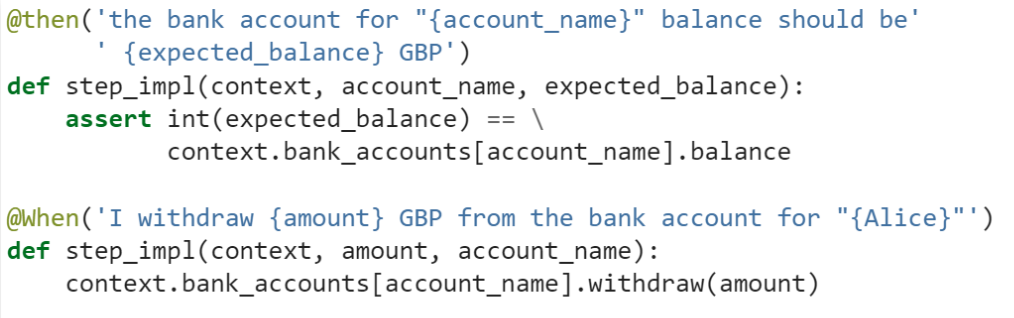
\includegraphics[scale=0.5]{src/11 BDD parametrised step fn.PNG}
\end{figure}
\noindent Note that parameters of the scenario become parameters of the function. We are using quotation marks around the parameters so that the regular expression used to match the step name is not overmatching the parameter.

\subsection{Step Abstraction}
Step abstraction is not a feature of Gherkin, but is present in Behave and JBehave. It allows us to denote complex steps by multiple simpler ones. It gives more flexibility than backgrounds by avoiding duplication of a sequence of steps. An example of this is given in Behave.
\begin{figure}[H]
    \centering
    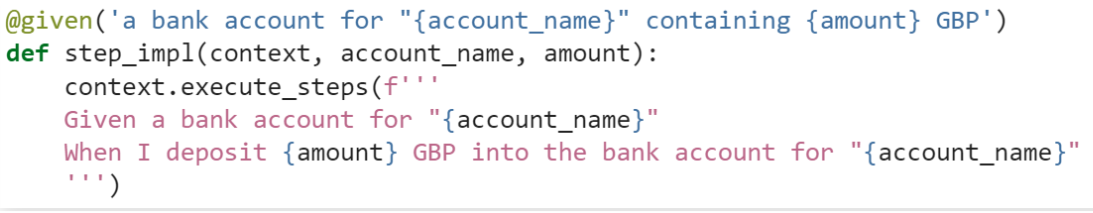
\includegraphics[scale=0.5]{src/11 BDD abstraction.PNG}
\end{figure}
\noindent In the example, we can executed steps from within the implementation function. This means that the explicitness of the step is lost from the feature file. Moreover, it often violates the step order, e.g. the when step is already included in the given step, so if there was an and step, it would be out of order.

\subsection{Scenario outlines and example tables}
We can use scenario outlines when the same sequence of steps can lead to different outcomes depending on the value of the input parameters. These are realised by an example table, as shown below.
\begin{figure}[H]
    \centering
    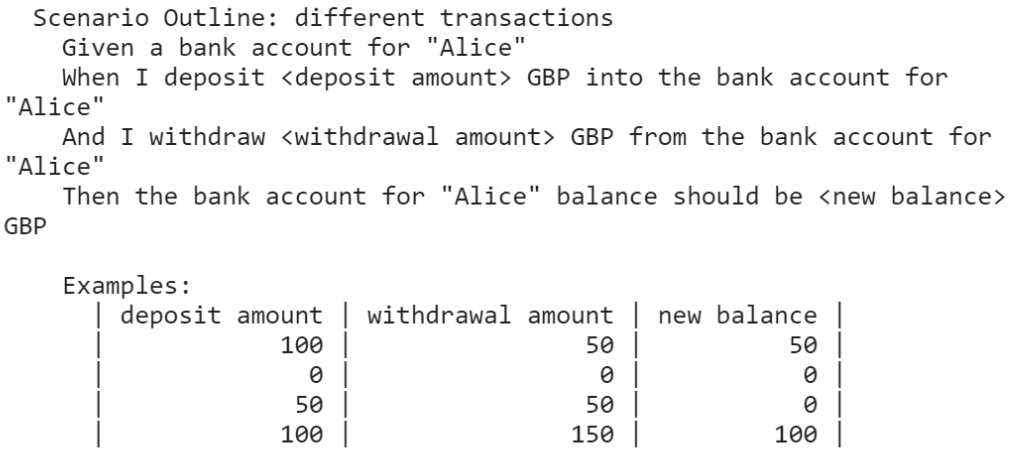
\includegraphics[scale=0.5]{src/11 BDD Scenario Outline and Example Tables.PNG}
\end{figure}
\noindent In the figure above, the value of new balance depends on the deposit amount and the withdrawal amount. We convert each row into a test case.

This feature is different to parametrised step functions, and is used in conjunction with it. In particular, the table generates lots of hard coded scenarios from a single scenario outline. In theory, all of these scenarios can be realised by different step functions, but they would be very similar. So, it makes sense to use parametrised step functions to realise the individual steps. For example, the parametrised step function in Behave for the example above is given below.
\begin{figure}[H]
    \centering
    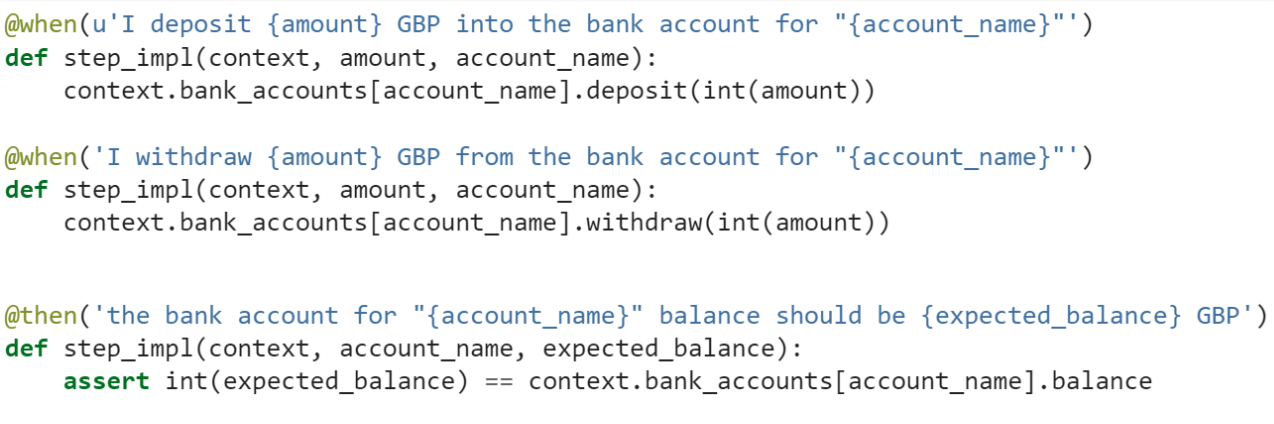
\includegraphics[scale=0.4]{src/11 BDD Python parametrised for scenario outline.PNG}
\end{figure}

\subsection{Level of testing in BDD}
In the example above, the desired behaviour is directly tested against the functional classes of the application rather than against the user interface. Some approaches to BDD use test suites that exercise the application via a user interface (or a REST API). In principle, this may be more desirable. In this case, the tests are being executed against the whole system as observed by a real user. 

However, this is difficult to do in practice. It can crease the cost considerably. Tests need to be adjusted as we make relatively minor changes to the user interface even when the business logic has not changed. We might even need to change it when the underlying frameworks change.

There are some tools that have been created to mitigate this problem, e.g. Selenium and Katalon tools for web app testing. We also have explicit extensions to BDD tools in many frameworks, such as django-behave.

\subsection{Good BDD practices}
It is a good practice to keep BDD scenarios short. We can use abstraction to mitigate longer scenarios. We should also keep the individual steps short. If the steps are long, we could probably break it into shorter steps that are easier to understand. We should comply with the AAA (arrange, at, assert) convention by having given, when, then structure. We should write features in the user-domain language. In particular, we should avoid using technical terms.

We should use a BDD framework to cut down on redundancy. We tend to develop features and implement them gradually instead of following the top-down approach (feature \texttt{->} scenario \texttt{->} steps). It is important to work closely with the customer to validate the features throughout the project rather than doing it at the end.

\subsection{Managing BDD}
BDD has many limitations. In L.P. Binamungu, et al (2018), there was a survey conducted with practitioners on the challenges in maintaining BDD specification. The paper identified many challenges:
\begin{itemize}
    \item Since we are using specification by example, we need to demonstrate every desired behaviour with an example. This can lead to lots of examples of the specification. This gets hard to manage as the specification grows.
    \item The philosophy of BDD advocates concrete examples, which makes abstraction and brevity difficult. In particular, it can be difficult to provide succinct specifications using this approach.
    \item There is an ongoing need to maintain consistency in step definitions as the specification and the API change. That is, when we change the specification or the API, we will need to update the step definitions to reflect this.
    \item BDD requires hard coding of dependencies in the `given' step. 
    \item There is only one level of abstraction possible in Gherkin, meaning that lots of duplicate sequences of steps can be present. Typically, this cannot be mitigated by techniques such as background.
    \item Gherkin steps are implicitly sequential, i.e. there is an order to them. So, we need to express all the possible orders in our scenarios, even when the order doesn't matter. For example, the order in which we enter the username and the password in a web application doesn't matter. But, to test that either combination works, we need to test both of the combinations. This further increases the size of the specification.
\end{itemize}

In summary, BDD provides a means through executable steps of ensuring traceability between the user facing requirements and implementations.

\end{document}